
\documentclass{article}
\usepackage[utf8]{inputenc}
\usepackage{graphicx}
\usepackage{geometry}
 \geometry{
	 a4paper,
	 total={170mm,257mm},
	 left=20mm,
 	top=20mm,
 } 
 
\title{DU@UP ObjectSensor and Mobile Navigation \\
The Inevitables
}

\author{  
            Peter Rayner\\
            Dawie Pritchard\\
            Drew Langley\\
            Hendrik Jan van der Merwe\\
            Lyle Nel\\
        }


\begin{document}

\maketitle

\newpage

\tableofcontents

\newpage


\section{Proposed Solution}

\subsection{Technologies}
\begin{itemize}
	\item J2EE 
		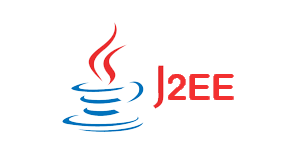
\includegraphics[width=5cm,height=5cm,keepaspectratio]{j2ee-logo.png} \\
	Java Enterprise Environment will be our main platform of development. It is a collection of Java APIs that software developers can use to write server-side applications.
	It consists of HTTP client technologies, Database and resource access technologies, REST and web service technologies, Java EE security and container management.
	All of which will be usable within the implementation of object sensor and mobile navigation.
	\item JDBC
		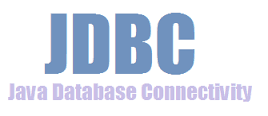
\includegraphics[width=5cm,height=5cm,keepaspectratio]{jdbc.png} \\
	JDBC is an API for java which defines how a client may access a database. it is part of the Java Standard edition platforms and provides methods to update data and query within a database.
	\item JPA
		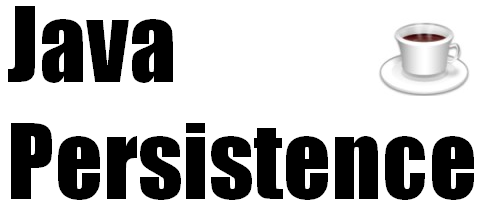
\includegraphics[width=5cm,height=5cm,keepaspectratio]{jpa.PNG} \\
	Java Persistence API is a java specification for accessing, persisting and managing data between java objects/classes
	JPA is considered the standard industry approach for Object to relational mapping in the java Industry.
	\item wildfly 10
		
\includegraphics[width=5cm,height=5cm,keepaspectratio]{wf.png} \\
	Wildfly is an application server authored by Jboss. Wildfly is written in java and implements the Java Platform,Enterprise Edition(JavaEE) specification and can run on multiple platforms.
	\item MongoDB
		
\includegraphics[width=5cm,height=5cm,keepaspectratio]{mongo.png} \\
	MongoDB is a cross platform and open source document-oriented database. It is a NoSQL database and uses BSON(JSON like documents that have dynamic shcemas). This is for massive amounts of information that could potentially be stored within the database.
\end{itemize}
N
\end{document}